%! Author = danielmendes
%! Date = 05.01.25
\chapter{Grundlagen}\label{ch:grundlagen}

In diesem Kapitel betrachten wir die Grundlagen der Bachelorarbeit, die in den späteren Kapiteln für die Durchführung der Benchmark-Tests und Analysen erforderlich sind.
Zunächst werden die Auswahl der einzelnen Tools, ihre Funktionsweise und die jeweiligen Vor- und Nachteile evaluiert.
Anschließend werden die einzelnen Schritte dargelegt, um die Tools korrekt zu verwenden.
Besonders beim Benchmark-Tool untersuchen wir die verschiedenen Argumente, die übergeben werden können und zeigen anhand eines kurzen Beispiels, wie die Resultate dieses Tools aussehen könnten.
Danach betrachten wir eine komplexere Demonstration, die wir zu großen Teilen bei späteren Tests wiederverwenden können.
Zu guter Letzt zeigen wir, wie GitHub Actions funktionieren, uns bei den Benchmark-Tests Aufwand ersparen und wie wir die Workflows sowohl zeitlich als auch ressourcenschonend optimieren können.

\section{Auswahl der Tools}\label{sec:auswahl-der-tools}

Zunächst gilt es, ein geeignetes relationales Datenbankmanagementsystem auszuwählen.
Die Entscheidung fiel auf MySQL, konkret auf die Version 8.0, die am 19.\ April 2018 mit der Veröffentlichung von Version 8.0.11 eingeführt wurde (\cite{mysql_release}).
Seitdem wird sie kontinuierlich weiterentwickelt, zuletzt mit 8.0.41 am 21.\ Januar 2025.
Daher wird auch der Schwerpunkt im weiteren Verlauf dieser Arbeit überwiegend auf MySQL liegen.

Die Grundlage dieser Bachelorarbeit ist das Verhalten der MySQL-Datenbank (\cite{sysbench_mysql}) in Bezug auf die unterschiedlichen Konzepte und Strategien, die später behandelt werden.
Das Ziel ist, dieses Verhalten mithilfe von Grafiken messbar und veranschaulicher zu machen.
Damit wir die Kennzahlen für bestimmte Abfragen an die MySQL–Datenbank bestimmen können, brauchen wir ein zentrales Tool.
Dieses Tool ist dafür verantwortlich, die Benchmark-Tests durchzuführen.
Meine Wahl ist schlussendlich auf \textbf{Sysbench} (\cite{sysbench_repo}) gefallen.

Sysbench ist ein Open-Source-Tool, das ein skriptfähiges, multi-threaded Benchmark-Tool ist, das auf LuaJIT basiert (\cite[pp. 50--66]{schwartz2012high}).
Es wird hauptsächlich für Datenbankbenchmarks verwendet, kann jedoch auch dazu eingesetzt werden, beliebig komplexe Arbeitslasten zu erstellen, die keinen Datenbankserver erfordern.
Dabei analysiert Sysbench Metriken, wie unter anderem Transaktionen pro Sekunde, Latenz und Anzahl an Threads.
Außerdem kann man genauer spezifizieren, wie oft diese Metriken geloggt werden sollen.
Sysbench ist nicht auf ein einziges Datenbanksystem beschränkt, da man sich für eines aus einer Liste verschiedener DBMS entscheiden kann.

Im Zuge der Wahl des Benchmark-Tools habe ich auch andere Benchmarking-Tools betrachtet, wie beispielsweise \textbf{Benchbase} (\cite{DifallahPCC13}) oder \textbf{mybench} (\cite{mybench_repo}).
Im Vergleich zu diesen Tools bietet Sysbench jedoch die Vorteile der höheren Skriptfähigkeit und Flexibilität.
Damit ist gemeint, dass die Verwendung von Sysbench im ersten Projekt aufwendiger ist, aber sobald ein Projekt einmal erstellt wurde, ist es sehr individuell anpassbar und schnelle Änderungen sind möglich.
Diesen Vorteil werden näher im Kapitel~\ref{sec:projektaufbau-mit-beispiel} veranschaulichen.
Dort werden wir den Einfluss unterschiedlicher Datentypen als Join-Operator zwischen zwei Tabellen vergleichen.
Wenn wir in einem späteren Kapitel die Performance verschiedener Indextypen analysieren, können wir viele Aspekte aus den Skripten der Join-Operatoren übernehmen.

Ein weiterer Vorteil von Sysbench ist, dass es als \textbf{de facto Standard} im Bereich der Datenbankbenchmarks angesehen wird (\cite{mybench_comparison}).
Durch diese Positionierung im Markt gibt es viele aktive Nutzer und dadurch bedingt viele verfügbaren Ressourcen.
Vorteile der anderen Tools sind jedoch die weniger präzise Steuerung der Ergebnisraten und der Transaktionen von Sysbench.
Zudem ist Sysbench auf das Minimale beschränkt, was den Output angeht, da es, wie schon erwähnt, nur eine Reihe von Log-Dateien ausgibt.
Außerdem muss die Visualisierung der Ergebnisse vom Benutzer selbst mithilfe von anderen Tools umgesetzt werden.
Anders sieht dies bei dem Tool mybench aus, da es dort die Möglichkeit gibt in Echtzeit umfassende Abbildungen zu betrachten (\cite{mybench_user_interface}).
Obwohl dieses Feature sehr hilfreich ist, bin ich nach Abwägung der Vor- und Nachteile zu dem Entschluss gekommen, dass die einfachere Bedienung und die Tatsache, dass Sysbench der de facto Standard ist, für mich überwiegen, weshalb ich mich für Sysbench entschieden habe.

Nichtsdestotrotz kann nicht komplett auf Graphen verzichtet werden.
Denn durch Abbildungen können Entwicklungen im Laufe einer Zeitmessung in einem Kurvenverlauf deutlich besser zu erkennen sind als in einer Log-Datei.
Anhand der reinen Zahlen in einem Log lassen sich unter Umständen Trends von zwei oder etwas mehr unterschiedliche Messungen erkennen, aber besonders zyklische Trends werden häufig ohne Visualisierung nicht schnell ersichtlich.
Wenn man aber Graphen mit einer Zeitachse hat, dann werden Trends sofort ersichtlich und auch der Vergleich unterschiedlicher Messungen erfolgt deutlich besser.

Um die Kennzahlen, die mithilfe von Sysbench ermittelt worden sind, in eine grafische Darstellung umzuwandeln, gibt es unterschiedliche Tools, die wiederum einige Vor- und Nachteile mit sich bringen.
Das erste mögliche Tool stellt Gnuplot~\cite{gnuplot} dar, mit dem sich CSV-Dateien sehr gut darstellen lassen.
Wenn man aber nur bestimmte Spalten aus der Tabelle darstellen will, kommt man schnell an seine Grenzen.
Deshalb habe ich mich mit einem Python-Script für eine anpassungsfähigere Alternative entschieden.
Für die grafische Darstellung sind dabei die Bibliotheken pandas (\cite{reback2020pandas}) und matplotlib.pyplot (\cite{hunter_2007}) verantwortlich.

\section{Einführung in die Tools}\label{sec:einfuhrung-in-die-tools}

Zuallererst muss der MySQL–Server gestartet sein.
Dabei ist es egal, ob dies lokal auf dem Rechner oder über einen Docker in eines GitHub CI/CD-Workflows erfolgt.
Das Wichtigste dabei ist es, dass man sich die Zugangsdaten, bestehend aus Benutzer- und Passwortdaten, speichert, da diese gebraucht werden, um den Benchmark-Test mit Sysbench zu starten.
Nachdem das RDBMS gestartet worden ist, muss zunächst eine Datenbank erstellt werden.
Das könnte beispielsweise folgendermaßen aussehen:

\vspace{-5pt}
\lstinputlisting[
    language=sql,
    label={lst:create_db},
    style=custom_daniel,
]{Scripts/Tools/01_database.sql}
\vspace{-5pt}

Zusätzlich zu erfolgreichen Erstellung der Datenbank muss das Tool Sysbench installiert werden.
Auf einem linux-basierten System kann Sysbench wie folgt installiert werden.
Wenn man das Betriebssystem macOS verwendet, muss \texttt{sudo apt-get} durch \texttt{brew} ersetzt werden.

\vspace{-5pt}
\begin{lstlisting}[language=bash]
sudo apt-get install sysbench
\end{lstlisting}
\vspace{-5pt}

Als Nächster machen wir uns näher mit dem Tool Sysbench vertraut.
Dazu gehen wir die verschiedenen Argumente, die beim Aufruf mitgegeben können oder müssen, durch und erklären sie kurz:

\begin{itemize}
    \setlength{\itemsep}{-0pt}
    \item \textbf{\texttt{db-driver}}: Treiber der Datenbank, in unserem Fall \textbf{\texttt{mysql}}
    \item \textbf{\texttt{mysql-host}}: Hostname oder IP-Adresse des Servers (Standard: \texttt{localhost})
    \item \textbf{\texttt{mysql-user}}: Benutzername der Datenbank
    \item \textbf{\texttt{mysql-password}}: Passwort des DB-Benutzers (kann weggelassen werden, wenn keine Authentifizierung erforderlich ist)
    \item \textbf{\texttt{mysql-db}}: Name der zu verwendenden Datenbank, bei uns: \textbf{\texttt{sbtest}}
    \item \textbf{\texttt{time}}: Laufzeit des Benchmarks in Sekunden und ist verpflichtend
    \item \textbf{\texttt{report-interval}}: Intervall in Sekunden, in dem Zwischenergebnisse angezeigt werden (Standard: nur Gesamtstatistiken am Ende)
    \item \textbf{\texttt{tables}}: Anzahl der zu erstellenden Tabellen (Standard: 1)
    \item \textbf{\texttt{table-size}}: Anzahl der Datensätze pro Tabelle (optional)
\end{itemize}

Neben den sieben aufgelisteten Argumenten gibt es zwei weitere wichtige Optionen:
\begin{enumerate}
    \item Wie im Abschnitt~\ref{sec:auswahl-der-tools} erwähnt, kann ein Lua-Skript angegeben werden, um eigene Tabellen zu erstellen, Beispieldaten einzufügen und bestimmte Abfragen durchzuführen.
    Dazu muss am Ende der Sysbench-Befehlszeile lediglich der Pfad zur Lua-Datei hinzugefügt werden.
    Ein erklärendes Beispiel dazu folgt weiter unten in diesem Abschnitt.
    \item Die Methode, den Sysbench ausführen soll, muss ebenfalls spezifiziert werden.
    Auch dieser wird am Ende der Sysbench-Befehlszeile angehängt.
\end{enumerate}

Um die korrekte Verwendung des Tools zu überprüfen, betrachten wir ein kurzes Demo-Beispiel, bei dem vordefinierte Testtypen von Sysbench genutzt werden.
Auf diese Weise kann man schnell kontrollieren, ob die Einrichtung des Tools korrekt ist, ohne dafür SQL-Befehle oder Lua-Skripte für die eigenen Bedürfnisse zu schreiben.
Es stehen verschiedene Testtypen zur Auswahl, wie das Einfügen von Daten (\textbf{oltp\_insert}), das Abfragen von Daten (\textbf{oltp\_read\_only}) oder beides (\textbf{oltp\_read\_write}).
Als Letztes müssen wir die unterschiedlichen Methoden auflisten, um sie mit den Testtypen kombinieren zu können:

\begin{itemize}
    \setlength{\itemsep}{-3pt}
    \item \textbf{prepare}: Bereitet die Datenbank für den Test vor, u.a.\ das Erstellen der Tabellen.
    \item \textbf{run}: Ist die Ausführungsphase des Tests.
    Je nach Testtyp führt diese Methode die spezifizierten Operationen aus, wie etwa \textbf{oltp\_read\_write}.
    Dabei wird die Performance der Datenbank unter der angegebenen Arbeitslast gemessen.
    \item \textbf{cleanup}: Diese Methode stellt die Datenbank in ihren ursprünglichen Zustand zurück und stellt sicher, dass keine Testdaten zurückbleiben.
\end{itemize}

Für unser Demo-Beispiel wählen wir den Testtyp \textbf{oltp\_read\_write} aus und kombinieren ihn mit allen Methoden.
Für die Methode \texttt{RUN} würde unsere Query so aussehen, wobei \texttt{YOUR\_USER} und \texttt{YOUR\_PASSWORD} durch die tatsächlichen Benutzerdaten der verwendeten Datenbank ersetzt werden müssten:

\vspace{-5pt}
\begin{lstlisting}[style=custom_daniel,label={lst:sysbenchrun}]
sysbench oltp_read_write \
  --db-driver=mysql \
  --mysql-user=YOUR_USER \
  --mysql-password=YOUR_PASSWORD \
  --mysql-db="sbtest" \
  --time=10 \
  --report-interval=1 \
  run
\end{lstlisting}
\vspace{-5pt}

Wenn man nur diese Query ausführt, fällt er auf, dass die Query scheitert.
Die Fehlermeldung lautet dabei wie folgt:

\begin{lstlisting}[style=custom_daniel,label={lst:error_withoutprepare}]
FATAL: MySQL error: 1146 "Table 'sbtest.sbtest1' doesn't exist"
\end{lstlisting}

Der entstandene Fehler wird offensichtlich dadurch verursacht, dass die Tabelle nicht erstellt worden ist.
Daher müssen wir vor der Ausführung der \texttt{RUN}-Methode zunächst die \texttt{PREPARE}-Methode durchführen.
Um die Datenbank wieder in den Ausgangszustand zu versetzen, muss nach dem \texttt{oltp\_read\_write}-Testtyp auch die \texttt{CLEANUP}-Methode aufgerufen werden.
Um sich die manuelle Ausführung dieser drei Befehle in der korrekten Reihenfolge zu sparen, bietet es sich an, ein Shell-Script zu schreiben, indem die Methoden nacheinander aufgerufen werden.

\vspace{-5pt}
\lstinputlisting[
    language=bash,
    caption=Ausführung der Sysbench-Methoden in korrekten Reihenfolge,
    label={lst:sysbench_monitor},
    style=custom_daniel,
    basicstyle=\ttfamily\scriptsize,
]{Scripts/Tools/02_process_sysbench.sh}
\vspace{-5pt}

Die Ergebnisse werden nun der Log-Datei (unter output/sysbench.log) gespeichert, aber uns fehlt noch die Erstellung der Graphen.
Um die Erstellung zu vereinfachen, bietet es sich an, die Kennzahlen aus der Log-Datei zu extrahieren und die Werte mit korrekten Spaltenüberschriften in einer CSV-Datei zu speichern.
Dies geht mit dem Shell-Kommando \texttt{grep}:

\vspace{-5pt}
\lstinputlisting[
    language=bash,
    caption=Extraktion der Ergebnisse aus der Log-Datei in eine Tabelle,
    label={lst:extraction_csv},
    style=custom_daniel,
    basicstyle=\ttfamily\scriptsize,
]{Scripts/Tools/03_extraction_csv.sh}
\vspace{-5pt}

Der letzte Schritt ist die Erstellung der Graphen mithilfe der Tools Gnuplot oder der Python-Library Pandas.
%TODO (Daniel): remove line underneath
Die kompletten Scripts \texttt{plot\_sysbench.gp} und \texttt{generatePlot.py} befinden sich am Ende dieser Bachelorarbeit.
Das Python-Script, das zuständig ist für die Visualisierung, muss als Argument zum einen die CSV-Datei übermittelt bekommen und zum anderen kann es nur eine bestimmte Auswahl an Messwerten übergeben, damit nur für diese die Graphen erzeugt werden.
In der Abbildung~\ref{fig:demo-graph-generation} können wir die Ergebnisse der Grapherstellung sehen.

\vspace{-5pt}
\lstinputlisting[
    language=bash,
    caption=Erstellung der Graphen aus der CSV-Datei,
    label={lst:graph_generation},
    style=custom_daniel,
    basicstyle=\ttfamily\scriptsize,
]{Scripts/Tools/04_graph_generation.sh}
\vspace{-5pt}

\vspace{-5pt}
\begin{figure}[H]
    \centering
    \begin{subfigure}[t]{0.36\textwidth}
        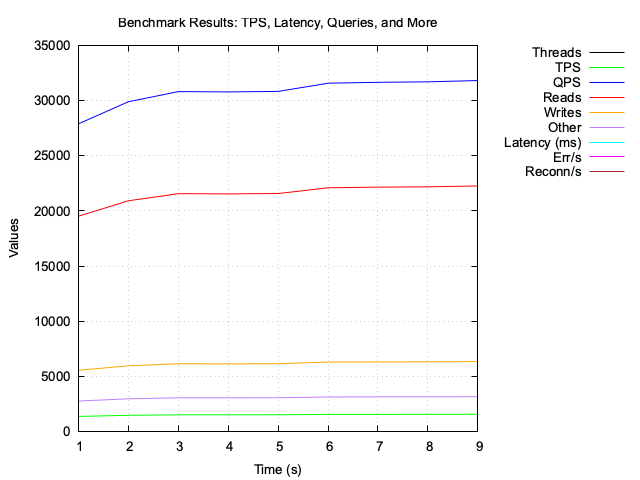
\includegraphics[width=\textwidth]{PNGs/Demo/sysbench_output}
    \end{subfigure}
    \hfill
    \begin{subfigure}[t]{0.48\textwidth}
        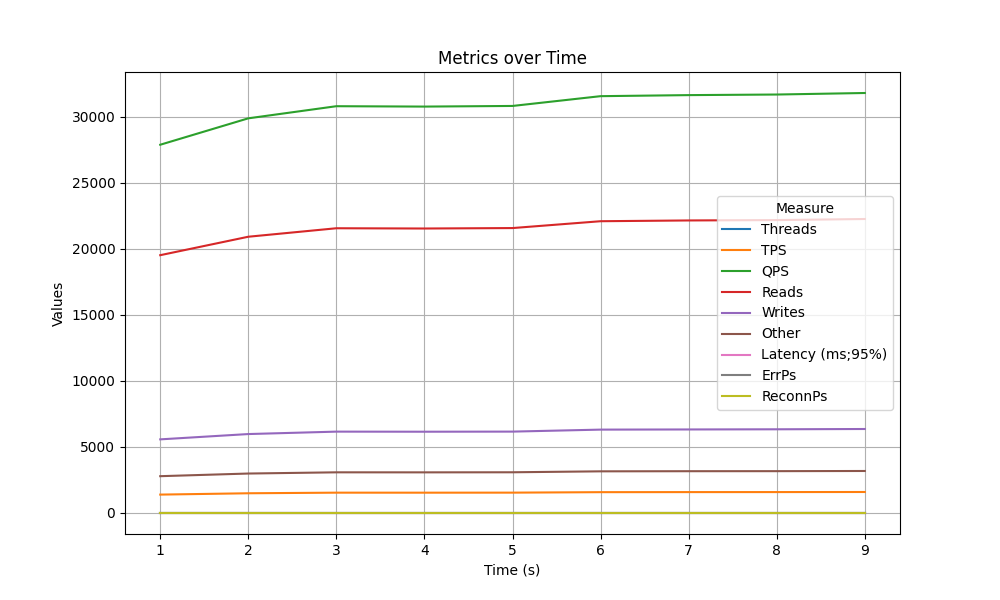
\includegraphics[width=\textwidth]{PNGs/Demo/Summary}
    \end{subfigure}
    \caption[Demo: Gnuplot vs. Pandas]{Grafik zeigt Erstellung mit Gnuplot (links) und Pandas (rechts)}
    \label{fig:demo-graph-generation}
\end{figure}
\vspace{-15pt}

Erklärung der einzelnen \textbf{Metriken}:
\begin{itemize}
    \setlength{\itemsep}{-5pt}
    \item \textbf{Threads}: Anzahl der gleichzeitig verwendeten Threads $\Rightarrow$ höhere Parallelität
    \item \textbf{TPS}: Transaktionen pro Sekunde; höherer Wert $\Rightarrow$ bessere Leistung
    \item \textbf{QPS}: Abfragen pro Sekunde; höherer Wert $\Rightarrow$ bessere Effizienz
    \item \textbf{Reads}: Anzahl der Leseoperationen; je mehr desto besser
    \item \textbf{Writes}: Anzahl der Schreiboperationen; je mehr desto besser
    \item \textbf{Other}: Andere Operationen, die weder als Reads noch Writes zählen
    \item \textbf{Latency (ms; 95\%)}: Durchschnittliche Bearbeitungszeit (im 95.\ Perzentil); \newline niedrigere Werte $\Rightarrow$ schnellere Reaktionszeiten
    \item \textbf{ErrPs}: Fehler pro Sekunde; niedriger Wert $\Rightarrow$ höhere Stabilität
    \item \textbf{ReconnPs}: Wiederverbindungen pro Sekunde; häufige Wiederverbindungen $\Rightarrow$ Hinweis auf Stabilitätsprobleme
\end{itemize}

\section{Projektaufbau mit Beispiel}\label{sec:projektaufbau-mit-beispiel}
In dem vorausgegangenen Kapitel \nameref{sec:einfuhrung-in-die-tools} wurde das Tool Sysbench und seine Funktionsweise anhand eines Demo-Projekts näher erläutert.
Damit die Reihenfolge und die Bedeutungen der unterschiedlichen Methoden (prepare → run → cleanup) sowie die Vorgehensweise zur Erstellung unserer Grafiken deutlich geworden.
Das bisherige Problem ist aber, dass wir bei dem dargelegten Beispiel keine Kontrolle über die getesteten Daten haben.
Wenn man sich die Logs genauer anschaut, dann sieht man, dass man über die Parameter an den Sysbench-Befehl die Anzahl der erstellten Tabellen und eingefügten Datensätze von außen steuern kann, aber die genaue Implementierung können wir auf diese Weise nicht steuern.
Genau für diese Anwendungsfälle gibt es die Möglichkeit ein Lua-Skript als Parameter beim Sysbench-Aufruf mit anzugeben.
In diesen Lua-Dateien können die Implementierungen der einzelnen Methoden selbstständig gewählt werden.

Um das Vorgehen besser erklären zu können, schauen wir uns dafür ein Beispiel an.
Für das Beispiel wollen wir zwei Tabellen erstellen und anschließend mit zufälligen Testdaten befüllen.
Die Abfrage, die wir auf Performance testen wollen, ist das Verbinden (Joinen) dieser beiden Tabellen.
In unserem Fall wollen wir eine Kundentabelle erstellen, die Informationen wie Name, Geburtstag und Adresse enthält, sowie eine Bestelltabelle, die Details wie Artikelnummer, Bestelldatum usw.\ speichert und einen Bezug zu dem Kunden herstellt, der die Bestellung aufgegeben hat.
Damit wir aber nicht nur ein Beispiel haben, das dargestellt wird, brauchen wir einen Vergleich zwischen zwei verschiedenen Implementierungen.
Dieser Unterschied zwischen den beiden Implementierungen besteht darin, dass in der einen Version die Tabelle eine Kundennummer vom Typ \texttt{Int} enthält, während in der anderen keine Kundennummer vorhanden ist.
Stattdessen wird in der Bestelltabelle auf den Namen (Typ \texttt{Varchar}) verwiesen.
Da Verbundoperationen zu den aufwendigsten Operationen gehören, gehen wir davon aus, dass der kleine Typ \texttt{Int} Performancevorteile gegenüber der anderen Version hat.
Dies gilt es nun mit den Benchmark-Test genauer zu untersuchen.

Für die Durchführung der Benchmarks beginnen wir zunächst unabhängig von Sysbench und den Lua-Skripten mit der Spezifizierung der Tabellen, die erstellt werden sollen.
Dies müssen wir einmal mit der Kundennummer und einmal mit dem Namen als Fremdschlüssel der Bestelltabelle machen.
Damit müssen insgesamt vier unterschiedliche Create Table-Befehle umgesetzt werden.
So sehen die Create Table für den Fall mit der Kundennummer aus:

\lstinputlisting[
    language=sql,
    caption=Create Table-Befehl für Tabelle Kunden,
    label={lst:create_table_kunde},
    style=custom_daniel,
    basicstyle=\ttfamily\scriptsize,
]{Scripts/Grundlagen/01_Create_Table_Kunde.sql}

\lstinputlisting[
    language=sql,
    caption=Create Table-Befehl für Tabelle Bestellung,
    label={lst:create_table_bestellung},
    style=custom_daniel,
    basicstyle=\ttfamily\scriptsize,
]{Scripts/Grundlagen/02_Create_Table_Bestellung.sql}

Anschließend müssen wir diese Befehle in \texttt{prepare()}-Funktion miteinbinden.
Dafür müssen wir einfach die Create Table-Befehle an die Datenbank senden.
Wenn wir bestimmte Indexe oder andere Datenbankstrukturen erstellen wollen würden, dann müssten wir dies ebenfalls in dieser Funktion machen.
Dies ist ein Auszug aus der \texttt{Prepare}-Funktion:

\lstinputlisting[
    language={[5.0]Lua},
    caption=Lua-Script für die Erstellung der Tabellen,
    label={lst:prepare_query},
    style=custom_daniel,
    basicstyle=\ttfamily\scriptsize,
]{Scripts/Grundlagen/03_Prepare_Query.lua}

Wenn die Datenbank beispielsweise in einer Produktivumgebung läuft, dann wollen wir, dass die Benchmarks möglichst wenig Einfluss auf sie haben.
Damit ist es das Ziel, dass die Datenbank möglichst wieder in ihrem Anfangszustand ist.
Außerdem sollte der Benchmark beliebig oft nacheinander ausgeführt werden können, ohne zu Problemen zu führen.
Wenn wir aber eine Tabelle erstellen und nicht wieder löschen, dann würde im nächsten Durchlauf der Create Table-Befehl scheitern.
Lösen könnte man dies über Klausel „IF NOT EXITS“ bei der Erstellung der Tabelle hinzufügen oder noch es besser ist es die Tabelle am Ende des Benchmarks einfach zu löschen.
Dafür ist die \texttt{cleanup()}-Funktion vorgesehen:

\lstinputlisting[
    language={[5.0]Lua},
    caption=Lua-Script für das Aufräumen,
    label={lst:cleanup_query},
    style=custom_daniel,
    basicstyle=\ttfamily\scriptsize,
]{Scripts/Grundlagen/04_CleanUp_Query.lua}

Wichtig ist dabei, dass man keine Schlüsselintegritäten verletzt.
Da in diesem Fall die Tabelle \texttt{BESTELLUNG} eine Referenz auf die Tabelle \texttt{KUNDEN} hat, muss zuerst die Bestelltabelle und danach erst die Kundentabelle entfernt werden.

Jetzt haben wir das Gerüst für die eigentlichen Insert- und Select-Befehle geschaffen.
Bei den Insert-Befehlen können wir entweder mit zufälligen Zahlen die Werte generieren oder wir setzen Listen von Namen fest, aus denen zufällig gewählt werden kann.
Da wir jedoch keine Kontrolle über diese zufällig erstellten Werte haben, müssen wir beim Insert-Befehl die Bedingung „Insert Ignore“ hinzufügen, damit doppelte Schlüsselwerte ignoriert werden und keine Fehler verursachen.
Wir müssen hier auch festlegen, wie viele Datensätze für die Kunden erstellt werden und wie viele Bestellungen pro Kunden es geben soll.
Später werden wir noch eine Möglichkeit kennenlernen, um diese Werte von außen zusteuern.
Um sicherzustellen, dass keine Werte in den Tabellen enthalten sind, können wir alle Datensätze aus den Tabellen entfernen, bevor wir sie hinzufügen.
Damit die Performance der Insert-Query auch gemessen wird, ist es wichtig, dass die \texttt{insert()}-Funktion in der \texttt{event()}-Funktion aufgerufen wird.
Sonst kommt es zu diesem Fehler:
\begin{lstlisting}[style=custom_daniel,label={lst:error_withoutevent}]
FATAL: cannot find the event() function in Join.lua
\end{lstlisting}

\lstinputlisting[
    language={[5.0]Lua},
    caption=Lua-Script für das Einfügen von Daten,
    label={lst:insert_query},
    style=custom_daniel,
    basicstyle=\ttfamily\scriptsize,
]{Scripts/Grundlagen/05_Insert_Query.lua}

Die letzte Anweisung, die wir noch brauchen, ist die Select-Abfrage.
Hierbei muss man sich Gedanken machen, welche Abfrage benötigt wird, damit die untersuchten Effekte auch tatsächlich auftreten.
In dem Beispiel brauchen wir deswegen einen Join zwischen den beiden Tabellen über den Fremdschlüssel.

\lstinputlisting[
    language={[5.0]Lua},
    caption=Lua-Script für das Abfragen von Daten,
    label={lst:select_query},
    style=custom_daniel,
    basicstyle=\ttfamily\scriptsize,
]{Scripts/Grundlagen/06_Select_Query.lua}

Damit haben wir für unseren Vergleich alle vier Operationen genauer definiert und müssen diese 4 Funktionen nur noch leicht anpassen für die Implementierung mit dem Namen als Fremdschlüssel und ohne die Kundennummer in der Kundentabelle.
Daraufhin benötigen wir noch ein Skript, dass die Operationen in der korrekten Reihenfolge ausführt und die Grafiken generiert.
Wichtig dafür ist die folgende Dateienstruktur, die anhand der Int-Verbunds dargestellt wird.

Damit wir die unterschiedlichen Operationen voneinander trennen können, gibt es folgende Dateienstruktur: Es gibt einen Ordner mit einem beliebigen Namen, z.B. \texttt{int\_queries}, in diesem Ordner befinden sich folgende Dateien:
\begin{itemize}\label{files_structure}
    \item \texttt{int\_queries.lua} $\Rightarrow$ enthält die \texttt{prepare()}- und \texttt{cleanup()}-Funktionen
    \item \texttt{int\_queries\_insert.lua} $\Rightarrow$ enthält die \texttt{insert()}-Funktion
    \item \texttt{int\_queries\_select.lua} $\Rightarrow$ enthält die \texttt{select()}-Funktion
\end{itemize}

Analog muss auch ein Ordner für die Varchar-Vergleich erstellt werden.
Als Letztes brauchen wir nur einen Orchestrator, der das korrekte Lua-Skript ausführt, die Ergebnisse in die richtige Log-Datei schreibt und anschließend die CSV-Dateien und die Grafiken erstellt.
Dieser Orchestrator ist das Shell-Skript: \texttt{sysbench\_script.sh}.

Zudem möchten wir unser Beispiel erweitern, da es auch möglich sein soll, unterschiedliche Längen von Varchar hinzuzufügen.
Dadurch könnten wir nicht nur den Performanceunterschied zwischen Int und Varchar feststellen, sondern auch noch den Einfluss der Länge des Verbundoperators für Varchar.
Dazu benötigen wir eine Hilfsfunktion in \texttt{varchar\_queries\_insert.lua}, die einen zufälligen Namen mit der Länge von einer vorgegebenen Zahl erstellt.
Dieser Name ist damit kein natürlicher Name, sondern einfach eine Kombination von zufälligen Buchstaben, aber für unseren Testfall gehen wir diesen Kompromiss ein.
Wenn wir jetzt zwei unterschiedlichen Längen für Varchar testen wollen, dann müssten wir den Varchar-Ordner mit den oben beschriebenen drei Dateien kopieren und nur die Zeile ändern, die die Länge des zufälligen Namens bestimmt.
Dies würde zu extremer Redundanz führen, weshalb man beim Aufruf des Orchestrator-Scripts, Variablen definieren kann, die im Skript selbst exportiert und in der \texttt{varchar\_queries\_insert.lua}-Datei importiert werden können.

Dies ist die Zeile mit der festgelegten Länge:
\begin{lstlisting}[language={[5.0]Lua},label={lst:without_imported_length,style=custom_daniel}]
local length = 10
\end{lstlisting}

Die Zeile mit der importierten Länge:
\begin{lstlisting}[language={[5.0]Lua},label={lst:with_imported_length,style=custom_daniel}]
local length = tonumber(os.getenv("LENGTH"))
\end{lstlisting}

Den Orchestrator-Script ruft man wie folgt auf:
\lstinputlisting[
    language=sh,
    caption=Befehl zum Ausführen des Orchestrator Skripts,
    label={lst:orchestrator_command},
    style=custom_daniel,
]{Scripts/Grundlagen/07_Orchestrator_Command.sh}

Die Parameter haben folgende Funktion:
\begin{itemize}[label=--]
    \item \texttt{-out}: Gibt den Pfad an, an welchen der Output-Ordner gespeichert werden soll
    \item \texttt{-var}: Angabe der Variablen und deren Werte, die exportiert werden sollen im JSON-Format
    \item \texttt{-scripts}: Angabe der Pfade zu den Ordnern, die die Lua-Skripte enthalten.
    Nach dem Doppelpunkt wird angegeben, welche Variable das Skript benötigt. \texttt{Int\_queries} benötigt keine Variablen, deshalb gibt es auch keinen Doppelpunkt.
\end{itemize}

Die letzte Besonderheit ist es, dass man mehrere Select-Abfragen ohne unterschiedliche Insert-Befehle definieren kann.
Zu einem späteren Punkt in der Bachelorarbeit werden wir zu unterschiedliche Indextypen kommen.
Um zu untersuchen, ob ein bestimmter Indextyp bei Abfragen verwendet wird, müssen wir nur unterschiedliche Selects abfragen.
Die eigentlichen Tabellen und deren Datensätze müssen dabei nicht immer wieder gleich befüllt werden.
Wenn wir auch unsere Ordnerstruktur mit dem Int-Query Beispiel zurückkommen, dann könnte man anstelle von \texttt{int\_queries\_select.lua} auch einen Ordner erstellen mit den Namen \texttt{int\_queries\_select}.
In diesem Ordner können beliebig viele unterschiedliche Lua-Skripts sein, die Select-Funktionen haben.
Dadurch werden alle Select-Befehle auf der gleichen Datenbasis verglichen und so können wir im Kapitel~\ref{sec:indexing-grundlagen} erkennen, wann der Index verwendet wird und wann nicht.

Bevor wir uns das Ergebnis des Befehls anschauen, kommen wir zu der Funktionsweise des Orchestrator-Skript \texttt{sysbench\_script.sh}.
Im Grundlegenden arbeitet dieses Skript ähnlich wie schon das Skript im Demo-Beispiel, aber durch die zusätzlichen Anwendungsfälle kommt es zu mehr Komplexität.

Zu Beginn des Skripts werden die Umgebungsvariablen aus der Datei \texttt{db.env} geladen.
Die Variablen helfen zum einen wie bei dem Demo-Beispiel bei der Datenbank-Verbindung und zum anderen können sich auch die Parameter der Benchmarks verändern.
Danach werden die Parameter, die an das Skript übergeben wurden, überprüft.
Beispielsweise wird sichergegangen, dass die für die Skripts verwendeten Parameter, bei unserem Beispiel length für varchar, tatsächlich auch definiert worden sind mit \texttt{-var}.

Wenn wir den Befehl ausführen, wird der Output-Ordner an der gewünschten Stelle erstellt.
In diesem Ordner werden verschiedene Grafiken generiert, die die Ergebnisse visualisieren.
Dabei gibt es zwei unterschiedliche Arten von Grafiken.
Die erste Art von Grafik ist ein Zeitreihendiagramm, welches auf der x-Achse den zeitlichen Verlauf zeigt.
Auf der y-Achse werden in einigen Diagrammen die unterschiedlichen Metriken für jedes einzelne Skript dargestellt, während andere Diagramme die Werte einer bestimmten Metrik auf der y-Achse zeigen und dabei die Ergebnisse verschiedener Skripte vergleichen.
Dadurch können beispielsweise die Metriken \texttt{Reads} und \texttt{Writes} analysiert werden, um herauszufinden, welches Skript in diesen Bereichen besser abschneidet.
Danach wird der Output-Ordner erstellt und die Spaltenüberschriften in die CSV-Dateien geschrieben.
Anschließend beginnt erst das eigentliche Durchgehen der unterschiedlichen Skripte, die unter dem Argument -script angegeben wurden.
Zunächst schreibt man die einzelnen Dateien nach dem obigen Schema (\ref{files_structure}) auf, denn als Argument wurde nur der oberste Ordner angegeben.
Als Nächstes kommt eine Fallunterscheidung, die überprüft, ob dieses Skript exportierte Variable nutzt oder nicht.
Für den Fall, dass keine Variablen exportiert werden (z.B. \texttt{int\_queries}) wird einfach die Prepare-Funktion aufgerufen, dann \texttt{process\_script\_benchmark} und anschließend die Cleanup-Funktion.
Wenn aber Variablen exportiert werden, dann müssen weitere Zwischenschritte umgesetzt werden.
Und zwar müssen alle Kombinationen zwischen den verschiedenen exportierten Variablen generiert werden.
Wenn es drei Variablen gibt, von denen 2 jeweils 2 Werte und eine letzte nur einen Wert hat, dann gibt es 2 × 2 × 1 = 4 unterschiedliche Kombinationen.
Als Nächstes muss man für alle diese Kombinationen die Schritte ausführen, die man schon bei der Variante ohne exportierte Variable ausgeführt hat und dabei darf man nicht vergessen die Variablen an sich zu exportieren.

\lstinputlisting[
    language=sh,
    caption=Ausschnitt aus Orchestrator Script,
    label={lst:main_loop},
    style=custom_daniel,
    basicstyle=\ttfamily\scriptsize,
]{Scripts/Grundlagen/08_Main_Loop.sh}

Die Funktion \texttt{process\_script\_benchmark} führt wie beim Demo-Beispiel schon erwähnt, die Methoden prepare, insert, selct und cleanup durch~\ref{lst:sysbench_monitor}.
Außerdem überprüft sie auch, ob es sich bei dem Select-Directory um einen Ordner handelt oder nicht.
Wenn es ein Ordner ist, dann werden alle Dateien in diesem Ordner mit Sysbench durchgeführt, wenn nicht, dann wird an den Ordner nur die Endung \texttt{.lua} hinzugefügt.

\lstinputlisting[
    language=sh,
    caption=Methode Process Script Benchmark,
    label={lst:process_script_benchmark},
    style=custom_daniel,
    basicstyle=\ttfamily\scriptsize,
]{Scripts/Grundlagen/09_Process_Script_Benchmark.sh}
\textbf{INFO:} Die Shell-Ausschnitte sind zum Teil verkürzt und würden auf diese Weise nicht funktionieren.

Die Methode \texttt{run\_benchmark} führt den Sysbench-Befehl (siehe~\ref{lst:sysbenchrun}) aus und nur wenn es sich um die Methode \texttt{RUN} handelt, werden die Daten während der Ausführung und die Endstatistiken in je eine CSV-Datei gespeichert.
Aus diesen beiden CSV-Dateien müssen die Insert-und Select-Queries der zugehörigen Skripte wieder vereint werden und die Attribute werden miteinander addiert.
Der letzte Schritt, der noch fehlt, ist die Erstellung der Graphen.

Wenn wir das komplette Skript für unser Join-Typ-Beispiel ausführen, dann ist das Endresultat ein Output-Ordner, der an angegebener Stelle erstellt wird.
In diesem Ordner werden verschiedene Grafiken generiert, die die Ergebnisse visualisieren.
Die erste Art stellen Zeitreihendiagramme dar, die auf der x-Achse den zeitlichen Verlauf zeigen.
Auf der y-Achse werden hingegen in einigen Diagrammen die unterschiedlichen Metriken eines einzelnen Skripts dargestellt, während andere Diagramme die Werte einer bestimmten Metrik auf der y-Achse zeigen und dabei die Ergebnisse verschiedener Skripte vergleichen.
Dadurch können beispielsweise die Metriken "Reads" und "Writes" analysiert werden, um herauszufinden, welches Skript in diesen Bereichen besser abschneidet.

Die zweite Art von Grafik, die erstellt wird, ist ein Hexagon-Diagramm.
Dieses verzichtet auf eine Zeitachse und fasst die Performance über den gesamten Zeitraum hinweg zusammen.
Im Vergleich zur Laufzeitanalyse liefert es zusätzliche Informationen, wie etwa die Latenz oder die Gesamtanzahl der Queries.
Dadurch ist es auch möglich, dass mehrere Skripte und mehrere Kennzahlen in einer Grafik dargestellt werden können.

\begin{figure}[H]
    \centering
    \begin{subfigure}[t]{0.48\textwidth}
        \centering
        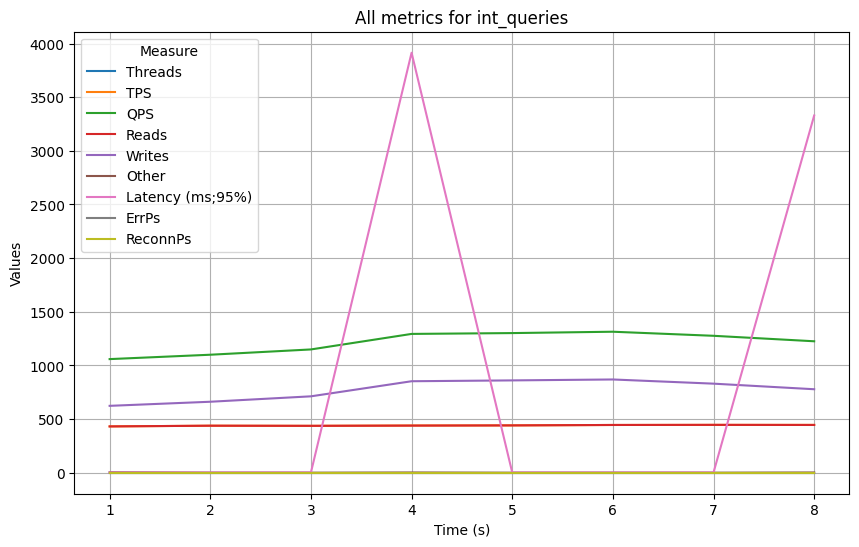
\includegraphics[width=\textwidth]{PNGs/Join_Type/int_queries}
        \caption{\texttt{int\_queries}}
        \label{join-typ-int_queries}
    \end{subfigure}
    \hfill
    \begin{subfigure}[t]{0.48\textwidth}
        \centering
        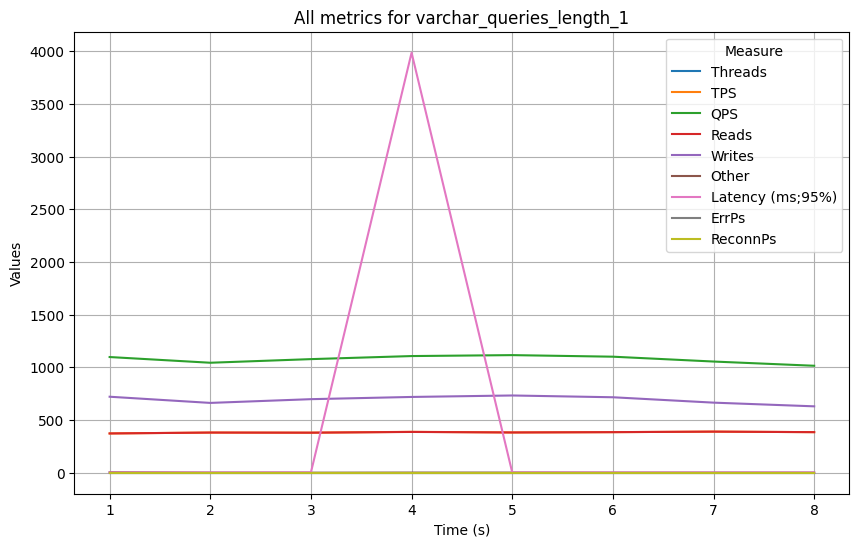
\includegraphics[width=\textwidth]{PNGs/Join_Type/varchar_queries_length_1}
        \caption{\texttt{varchar\_queries\_length\_1}}
        \label{join-typ-varchar_queries_length_1}
    \end{subfigure}
    \caption[Join-Typ: Skriptvergleich]{Die Grafik zeigt alle Metriken für die jeweiligen Skripte}
    \label{fig:join-typ-comp-script}
\end{figure}
\vspace{-20pt}

Aus den Grafiken, die für ein Skript alle Metriken veranschaulichen, kann man möglicherweise Datenfehler erkennen.
So springt bei Abbildung (\texttt{int\_queries.png}) die Latenz bei einigen Messpunkten von 0 ms auf einen deutlich erhöhten Wert und danach wieder auf 0 ms zurück.
Ansonsten aber sind die anderen Metriken auf einem konstanten Level und es gibt wenige Schwankungen.
Bei der Abbildung (\texttt{varchar\_queries\_length\_1.png}) sieht dies sehr ähnlich aus und auch dort schwankt die Latenz etwas mehr.
Wenn wir jetzt die drei Skripte miteinander vergleichen wollen, können wir die Abbildungen Reads.png und Writes.png heranziehen.
Was die Lesegeschwindigkeit angeht, kann man erkennen, dass \texttt{int\_queries} am meisten Reads hat, als Nächstes kommt \texttt{varchar\_queries\_length\_1} und dann \texttt{varchar\_queries\_length\_64}.
Damit sind die Abfragen, wie wir erwartet haben, bei \texttt{int\_queries} am schnellsten und je länger der String wird, desto langsamer werden die Abfragen.
Bei den Schreibgeschwindigkeiten sieht das schon etwas anders aus, wobei es hier zunächst bei allen eine langsamere Startphase gibt.
Anschließend an diesen Cold Start liegt das Niveau von \texttt{int\_queries} am höchsten, also auch am schnellsten.
Die beiden \texttt{varchar\_queries} sind hier aber überraschenderweise auf einem ähnlichen Niveau.

\begin{figure}[H]
    \centering
    \begin{subfigure}[t]{0.48\textwidth}
        \centering
        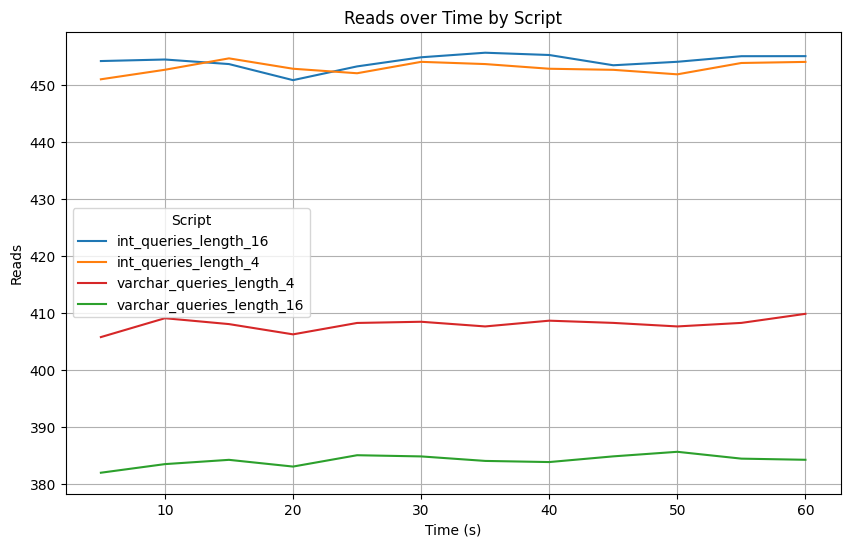
\includegraphics[width=\textwidth]{PNGs/Script/Join_Typ/join-type/Reads}
        \caption{Reads}
        \label{join-typ-reads}
    \end{subfigure}
    \hfill
    \begin{subfigure}[t]{0.48\textwidth}
        \centering
        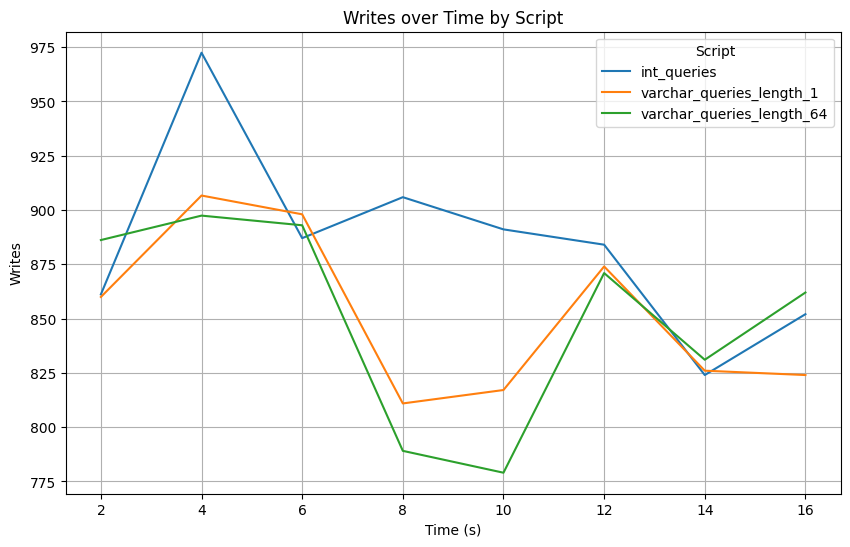
\includegraphics[width=\textwidth]{PNGs/Script/Join_Typ/join-type/Writes}
        \caption{Writes}
        \label{join-typ-writes}
    \end{subfigure}
    \caption[Join-Typ: Metrikvergleich]{Die Grafik zeigt den Vergleich zwischen allen Skripten für die Metriken}
    \label{fig:join-typ-comp-metric}
\end{figure}
\vspace{-20pt}

Bei der Abbildung (\texttt{statistics.png}) kann man die Effekte der Lese- und Schreibgeschwindigkeiten auch erkennen.
Es fällt auch auf, dass, anders als bei Reads, Writes, Queries, die Latenz bei schnelleren Queries geringer ist und nicht der höchste Wert der Beste ist.

\begin{figure}[H]
    \centering
    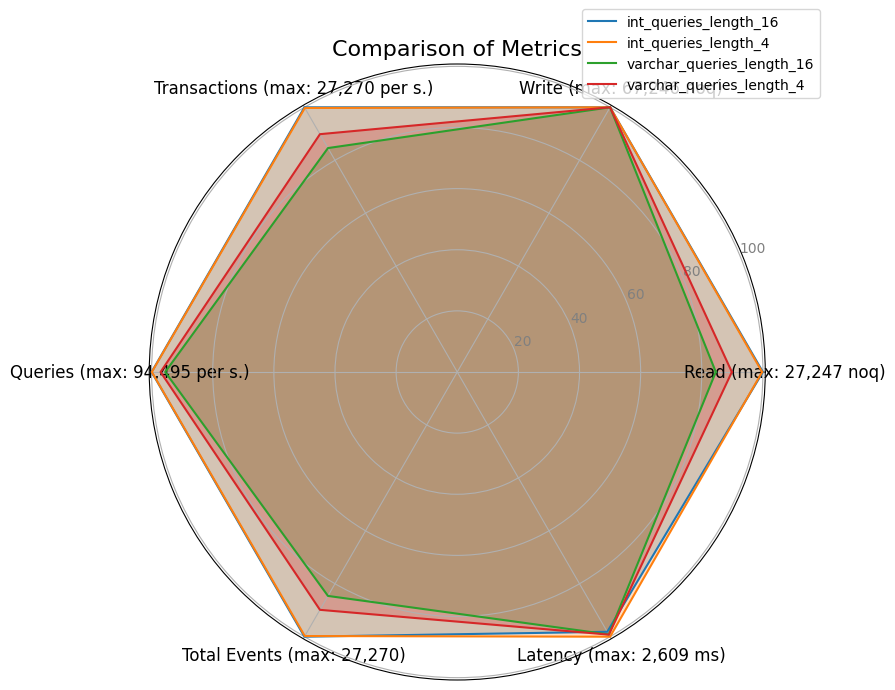
\includegraphics[width=.6\textwidth]{PNGs/Script/Join_Typ/join-type/statistics}
    \caption[Join-Typ: Hexagon-Diagramm]{Darstellung der Skripte und 6 Metriken in einem Hexagon}
    \label{fig:join-typ-hex}
\end{figure}

\section{GitHub Action}\label{sec:github-action}

Im Verlauf der Bachelorarbeit sind immer mehr unterschiedliche Projekte dazugekommen, wie in den späteren Kapiteln zu sehen sein wird, die alle das Orchestrator-Skript verwenden.
Dadurch sind immer mehr Fallunterscheidungen im Hauptskript erforderlich geworden und man hat schnell den Überblick verloren, wenn man Änderungen vorgenommen hat.
Um diese Änderungen zu überprüfen, mussten jedes Mal alle Skripte nacheinander ausgeführt werden, was nicht nur zeitintensiv war, sondern auch hohe Lasten für den lokalen Rechner bedeutete.
Eine Möglichkeit wäre es gewesen, die Skripte parallel durchlaufen zu lassen, um Zeit zu sparen, damit wäre aber nicht das Lastenproblem und der manuelle Aufwand gelöst worden.
Eine deutlich bessere Variante ist das Automatisieren dieser Befehle unabhängig von dem lokalen Rechner auf virtuellen Maschinen in der Cloud.
Als Plattform für diese Continuous Integration und Continuous Delivery (CI/CD) habe ich mich für GitHub Actions entschieden (\cite{github_action_doku}).
Mit GitHub Actions kann man Workflows erstellen, die bei einem bestimmten Event getriggert werden und anschließend eine Anzahl von Aufträgen nacheinander oder gleichzeitig ausführen können.
Jeder Auftrag (engl.\ Job) wird innerhalb eines eigenen Runners der virtuellen Maschine in einem Container ausgeführt und mann über einen oder mehrere Schritte (engl.\ Step) verfügen.
Die Schritte können wiederum beliebige Shell-Befehle, Skripte oder Aktionen ausführen.

Wie in den Kapiteln~\ref{sec:einfuhrung-in-die-tools} und~\ref{sec:projektaufbau-mit-beispiel} erklärt, müssen wir das Hauptskript ausführen, in dem die Benchmark-Tests durchführen werden.
Außerdem benötigen wir auch die Pfade zu den Lua-Skripten, die getestet werden sollen und in einigen Fällen müssen wir auch Variablen definieren, die später exportiert und in den Lua-Skripts verwendet werden.
Diese Pfade und Variablen müssen wir pro Projekt definieren und zusammen mit je einem Namen in einer JSON-Datei speichern.

\lstinputlisting[
    language=Json,
    caption=JSON mit Konfiguration der Script,
    label={lst:script_configuration},
    style=custom_daniel,
]{Scripts/Grundlagen/10_Pattern.json}

Damit wir das Hauptskript ausführen können, müssen wir im ersten Auftrag (engl.\ Job) die Daten dieser JSON-Datei verarbeiten und bestimmte Variablen, wie beispielweise den Output-Ordner definieren.
Zudem müssen wir alle Namen der verschiedenen Projekte in einer Liste zusammenfügen und als Output für den nächsten Job definieren.
Dieser Job wird erst gestartet, wenn der Erste beendet ist und ist verantwortlich für das eigentliche Durchführen der Benchmarks.
Da wir die Vorteile des gleichzeitigen Ausführens der Aufträge nutzen wollen, müssen wir die Matrixstrategie verwenden, damit die Benchmarks parallel ausgeführt werden.
Bei der Matrixstrategie kann man Variablen definieren, um automatisch mehrere Auftragsausführungen parallel zu erstellen.
In unserem Fall verwenden wir dafür die Liste mit den unterschiedlichen Projektnamen.

Damit nun die Benchmarks ausgeführt werden können, müssen wir innerhalb dieser Matrixausführung einige Vorbereitungen treffen.
Zum einen müssen wir die Dependencies für Sysbench und die Python-Libraries installieren und zum anderen müssen wir einen MySQL-Container mit passenden Konfigurationen starten und vorbereiten.
Nach diesen Schritten können wir das Hauptskript ausführen und die Outputdateien werden an dem angegebenen Pfad erstellt.

Um Zugriff auf diese Dateien zu erhalten, müssen wir sie als GitHub Artifact hochladen.
Die GitHub Artifacts können wir anschließend entweder über die GitHub REST Api oder die Übersicht des Workflows in GitHub als Zip-Datei herunterladen.
Als letzten Auftrag, nach Beendigung beider vorangegangenen Jobs, können wir alle GitHub Artifacts zu diesem Workflow herunterladen und gemeinsam als Artifact wieder hochladen, damit wir z.B.\ bei 10 Projekten, nicht 10 Zip-Dateien herunterladen und einzeln entpacken müssen, um die Änderungen der Dateien zu überprüfen.
Wenn fehlerhafte Änderungen den Workflow triggern, kann es dazu kommen, dass je nach Fehler unterschiedliche Jobs oder Steps nicht erfolgreich ausgeführt werden und damit der komplette Workflow scheitert.

Der Workflow wird in einer YAML-Datei im Ordner ~\texttt{.github/workflows/} definiert.
Zunächst muss man den Names des Workflows definieren und anschließend, wann er getriggert werden soll.
Dies kann beispielsweise manuell auf GitHub mit dem Tag \texttt{workflow\_dispatch} oder bei jedem Push mit \texttt{push}, u.a.\ kann das auch auf bestimmte Dateien oder Ordner einschränken.
Unter dem Tag \texttt{env} muss man die Umgebungsvariablen definieren, dazu gehören zum Beispiel der Datenbankname oder die Länge der Durchführung des Benchmarks.
Wenn es sich um vertrauliche Informationen handelt, sollte man GitHub Secrets dafür verwenden.
Ein Beispiel dafür wäre das Downloaden der Artefakte im letzten Job, um einen gemeinsamen Output-Ordner zu erstellen.
Dafür wird die GitHub REST API benötigt, die ein vertrauliches \texttt{Personal Access Token} erfordert, welches Repository- sowie Lese- und Schreibrechte für GitHub Registries besitzt.

\lstinputlisting[
    language=yaml,
    caption=Ausschnitt aus der Workflow-Datei,
    label={lst:workflow_yaml},
    style=custom_daniel,
    basicstyle=\ttfamily\scriptsize,
]{Scripts/Grundlagen/11_Workflow.yaml}

Die eben beschriebene YAML-Datei reicht aus, damit alle angegebenen Skripten in dem JSON ausgeführt und die Output Dateien alle korrekt in einem Ordner als ZIP-Datei hochgeladen werden.
Es bieten sich aber auch Alternativen an, die zu einer Optimierung des Workflows führen.

\section{Optimierungen des Workflows}\label{sec:optimierungen-des-workflows}

Zum einen kann man die zu installierenden Abhängigkeiten mithilfe des GitHub Caches (\cite{github_cache_doku}) speichern.
Dies bietet sich besonders an, da sich die Abhängigkeiten über die Workflows hinweg nur selten ändern.
Falls sich doch etwas ändert, kann man beispielsweise die \texttt{require\allowbreak ments.txt}-Datei anpassen.
Dadurch werden einmalig alle Abhängigkeiten neu installiert und anschließend im Cache abgelegt.
Falls sich bis zum nächsten Workflow keine Änderungen an den Abhängigkeiten ergeben, wird der Cache automatisch genutzt.
Der Zeitgewinn in unserem Beispiel ist jedoch nur gering und beträgt nur wenige Sekunden pro Workflow.

\lstinputlisting[
    language=yaml,
    caption=Speichern der Abhängigkeiten im Cache,
    label={lst:cache_yaml},
    style=custom_daniel,
]{Scripts/Grundlagen/12_Cache.yaml}

Deutlich mehr Zeit und Ressourcen kann man aber sparen, wenn man zwischen zwei unterschiedlichen Arten von Dateien unterscheidet.
Denn zum einen gibt es Dateien, die die Ergebnisse von allen Skripten beeinflussen.
Dazu gehören das Workflow-Skript und die JSON-Datei, aber auch das Orchestrator-Skript und die darin verwendeten Python-Skripte.
Die Ordner an sich, die in der JSON angegeben werden, die beeinflussen nur sich selbst und nicht die anderen Skripte.
Beispielweise, wenn ich in Projekt A die Anzahl an Zeilen ändere, die ausgeführt werden, dann ändert dies nichts an dem Ergebnis von Projekt B oder C\@.
In diesem Beispiel würde es sich anbieten, dass für Projekt A die Benchmarks neu durchgeführt werden, für Projekt B und C könnte hingegen jeweils der letzte erfolgreiche Output Ordner benutzt werden.
Als Endresultat könnten damit die neue Durchführung von Projekt A zusammen mit der alten Ausführung der Projekte B und C in einer Zip-Datei hochgeladen werden.
Dadurch wird nur ein Drittel der eigentlichen Ressourcen verbraucht, wenn man davon ausgehen würde, dass alle 3 Projekte gleich viel Zeit benötigen würden.

Für die Implementierung dieser Optimierung muss zunächst die allgemeinen Skripte hashen und zusätzlich noch die Ordner mit den Lua-Skripten, die für das jeweilige Skript aus der JSON benötigt werden.
Diese beiden Hashes kann zusammen mit den Testtypen kombinieren, damit bekommt die folgende Struktur für den Namen:

\begin{lstlisting}[language=yaml,label={lst:hash_name},style=custom_daniel]
NAME="${{ matrix.test-type }}-${{ env.hash }}-${{ env.general_hash }}"
\end{lstlisting}

Nachdem wir unsere JSON geladen haben, machen wir nun nicht mehr direkt mit der Installation der Abhängigkeiten weiter, sondern davor hashen wir die unterschiedlichen Pfade und erstellen unseren Namen.
Wenn es keinen Ordner mit dem gleichen Namen gibt, dann machen wir weiter wie bisher.
Das einzige, was sich ändert, ist der Schritt vor dem Hochladen des gesamten Output-Ordners.
Der vom Testtypen erzeugte Ordner muss zusammen mit seinem Namen hochgeladen werden, damit er im nächsten Workflow heruntergeladen werden kann, sofern die Hashes unverändert bleiben.
Ist dies beim nächsten Workflow der Fall, dann muss der Ordner nur heruntergeladen werden und and die korrekte Adresse im Output Ordner verschoben werden.
Die Installation der Abhängigkeiten, das Starten des MySQL-Containers und das Ausführen des Orchestrator-Skripts hat man sich damit erspart.

Die letzte Frage lautet, wo die Ordner mit den berechneten Namen gespeichert und beim nächsten Run wieder heruntergeladen werden sollen.
Zum einen kann man Lösungen in GitHub selbst verwenden.
Zum einen würde sich eine GitHub Cache-Lösung wieder anbieten, aber tatsächlich sind GitHub Artifacts für das Sichern von Dateien besser geeignet (\cite{github_cache_doku}).
Eine andere interessante Lösung kann auch das Nutzen von expliziten Branches nur für die Sicherung der Dateien seien.
Das Problem ist hier, dass es manchmal durch bestimmtes Timing zu Problemen beim Pushen kommen kann, da zufällig ein anderer paralleler Workflow in der Zeit zwischen Rebase, Commit und Push den Code verändert hat, wodurch nach verhindertem Push erneut ein Rebase durchgeführt werden muss.
Außerdem muss man dafür der GitHub Action Schreibberichtigungen geben.
Des Weiteren eignen sich auch Cloud-Speicherlösungen sehr gut, um die Ordner zu speichern und wieder herunterzuladen.
Dazu gehören von Google Cloud Storage (GCS), AWS S3 oder MS Azure Storage, die sich zusammen mit GitHub Artifacts am besten eignen.